\documentclass{standalone}
  \usepackage{amsfonts,amsmath,amssymb}
  \usepackage[slovene]{babel}
  \usepackage[utf8]{inputenc}
  \usepackage[T1]{fontenc}
  
\usepackage{tikz, verbatim, subcaption}
\usepackage{pgfplots}
\usetikzlibrary{arrows.meta, calc, positioning, automata}
\usetikzlibrary {decorations.pathreplacing}

\begin{document}

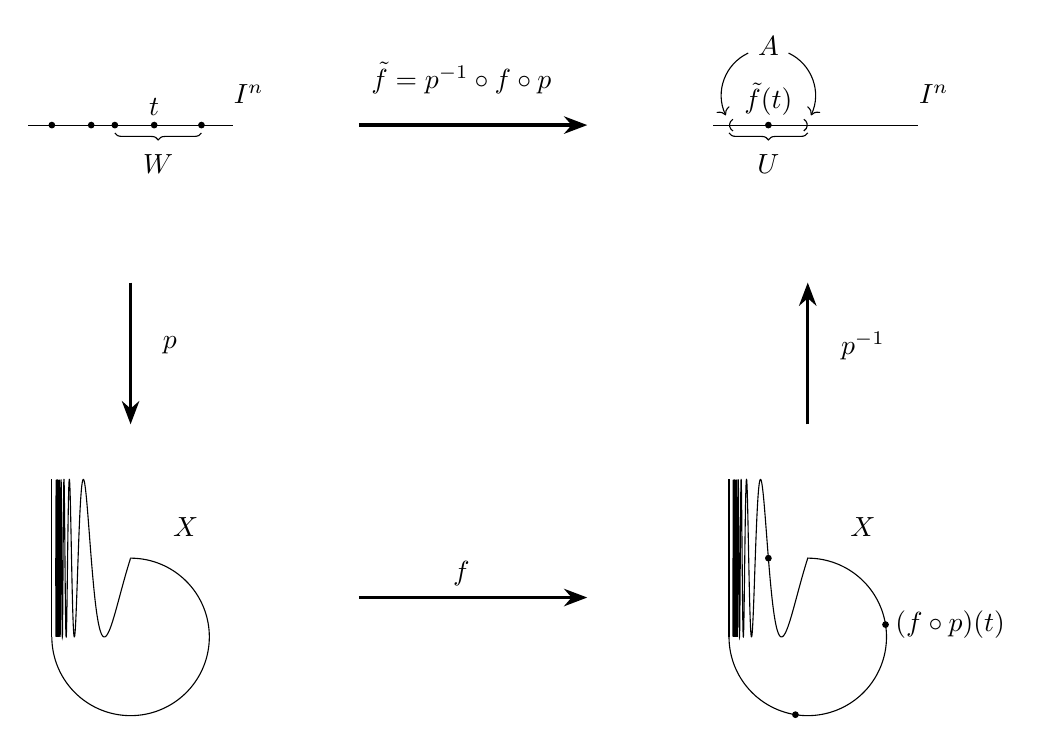
\begin{tikzpicture}[decoration=brace]
% ###############          levi interval          ###############
		\draw (-5.9, 3) -- (-3.3, 3);
		\draw (-3.1, 3.4) node {$I^n$};
		\filldraw (-4.3, 3) circle (1pt) node[black, above] {$t$};
		\filldraw (-5.6, 3) circle (1pt);
		\filldraw (-5.1, 3) circle (1pt);
		\filldraw (-4.8, 3) circle (1pt);
		\filldraw (-3.7, 3) circle (1pt);
		\draw [decorate] (-3.7,2.9) -- (-4.8,2.9);
		\draw (-4.25, 2.5) node {$W$}; 
		
% ###############          desni interval          ###############
		\node (A) at (3.5,4) {$A$};
		\node (x) at (3,3) {};
		\node (y) at (4,3) {};
		\draw (2.8, 3) -- (5.4, 3);
		\draw (5.6, 3.4) node {$I^n$};
		\draw[<->, > = {Parenthesis[]}] (3,3) -- (4,3) ;
		\filldraw (3.5, 3) circle (1pt) node[black, above] {$\tilde{f}(t)$};
		\draw [decorate] (4,2.9) -- (3,2.9);
		\draw (3.5, 2.5) node {$U$};  
		\draw [->] (A) to [bend left=45] (y);
		\draw [->] (A) to [bend right=45] (x);

% ###############          desna krožnica          ###############

		\draw (3,-3.5) -- (3,-1.5);
   % \draw[->] (0,-1) -- (0,1.1) node[above] {$\sin (1/x)$};
   		\draw[domain=3.05:4.001,samples=2000, smooth] plot (\x, {sin((pi/(\x-3))r)-2.5});
		\draw[domain=1:2.0025,samples=500, smooth] plot ({cos((3*pi*\x/2-pi/2)r)+4}, {sin((3*pi*\x/2-pi/2)r)-3.5});
		\draw (4.7, -2.1) node {$X$};
		\filldraw[] ({cos((3*pi*1.7/2-pi/2)r)+4}, {sin((3*pi*1.7/2-pi/2)r)-3.5}) circle (1pt) node[black, right] {$(f \circ p) (t)$};
		\filldraw[] ({cos((3*pi*1.3/2-pi/2)r)+4}, {sin((3*pi*1.3/2-pi/2)r)-3.5}) circle (1pt) node[black, above] {};
		\filldraw[] (3.5, {sin((pi/(0.5))r)-2.5}) circle (1pt) node[black, above] {};
 

		
% ###############          leva krožnica          ###############
		\draw (-5.6,-3.5) -- (-5.6,-1.5);
   % \draw[->] (0,-1) -- (0,1.1) node[above] {$\sin (1/x)$};
		\draw[domain=-5.55:-4.601,samples=2000, smooth] plot (\x, {sin((pi/(\x+5.6))r)-2.5});
		\draw[domain=1:2.0025,samples=500, smooth] plot ({cos((3*pi*\x/2-pi/2)r)-4.6}, {sin((3*pi*\x/2-pi/2)r)-3.5});
		\draw (-3.9, -2.1) node {$X$};
	
	
% ###############          puščice          ###############
		\draw [black, line width=1.2pt, -Stealth] (-1.7,3) -- (1.2,3);
		\draw (-0.4, 3.6) node {$\tilde{f} = p^{-1} \circ f \circ p$};
		\draw [black,  line width=1.2pt, -Stealth] (-1.7, -3) -- (1.2, -3);
		\draw (-0.4, -2.7) node {$f$};
		\draw [black,  line width=1.2pt, -Stealth] (-4.6, 1) -- (-4.6, -0.8);
		\draw (-4.1, 0.2) node {$p$};
		\draw [black,  line width=1.2pt, -Stealth] (4, -0.8) -- (4, 1);
		\draw (4.7, 0.2) node {$p^{-1}$};  
	\end{tikzpicture}
	
\end{document}